% -*- mode: LaTeX; TeX-PDF-mode: t; -*-  # Config emacs auctex
% Slides for presentation at the Norwegian University of Science and Technology, January 23, 2025.

% allow latex to find custom stuff
% Add the listed directories to the search path
% (allows easy moving of files around later)
% these paths are searched AFTER local config kpsewhich

% *.sty, *.cls
\makeatletter
\def\input@path{{@resources/texlive/texmf-local/tex/latex/}
        ,{@resources/texlive/texmf-local/bibtex/bst/},
        ,{@resources/texlive/texmf-local/bibtex/bib/},
        ,{@local/}
        }
\makeatother
\makeatletter
\def\bibinput@path{{@resources/texlive/texmf-local/tex/latex/}
        ,{@resources/texlive/texmf-local/bibtex/bst/},
        ,{@resources/texlive/texmf-local/bibtex/bib/},
        ,{@local/}
        }
\makeatother
  

% Set paths (like, \LaTeXInputs) to find resources
% -*- mode: LaTeX; TeX-PDF-mode: t; -*- 
% LaTeX path to the root directory of the current project
% from the directory in which this file resides
% and path to econtexPaths which defines the rest of the paths like \FigDir
\providecommand{\econtexRoot}{}\renewcommand{\econtexRoot}{.}
\providecommand{\econtexPaths}{}\renewcommand{\econtexPaths}{econtexPaths}
% -*- mode: LaTeX; TeX-PDF-mode: t; -*- 
% The \commands below are required to allow sharing of the same base code via Github between TeXLive on a local machine and Overleaf (which is a proxy for "a standard distribution of LaTeX").  This is an ugly solution to the requirement that custom LaTeX packages be accessible, and that Overleaf prohibits symbolic links
\providecommand{\packages}{\econtexRoot/Resources/texmf-local/tex/latex}
\providecommand{\econtex}{\packages/econtex}
\providecommand{\econark}{\econtexRoot/Resources/texmf-local/tex/latex/econark}
\providecommand{\econtexSetup}{\econtexRoot/Resources/texmf-local/tex/latex/econtexSetup}
\providecommand{\econarkSetup}{\econtexRoot/Resources/texmf-local/tex/latex/econarkSetup}
\providecommand{\econtexShortcuts}{\econtexRoot/Resources/texmf-local/tex/latex/econtexShortcuts}
\providecommand{\econtexBibMake}{\econtexRoot/Resources/texmf-local/tex/latex/econtexBibMake}
\providecommand{\econtexBibStyle}{\econtexRoot/Resources/texmf-local/bibtex/bst/econtex}
\providecommand{\econtexBib}{economics}
\providecommand{\notes}{\econtexRoot/Resources/texmf-local/tex/latex/handout}
\providecommand{\handoutSetup}{\econtexRoot/Resources/texmf-local/tex/latex/handoutSetup}
\providecommand{\handoutShortcuts}{\econtexRoot/Resources/texmf-local/tex/latex/handoutShortcuts}
\providecommand{\handoutBibMake}{\econtexRoot/Resources/texmf-local/tex/latex/handoutBibMake}
\providecommand{\handoutBibStyle}{\econtexRoot/Resources/texmf-local/bibtex/bst/handout}

\providecommand{\FigDir}{\econtexRoot/Figures}
\providecommand{\CodeDir}{\econtexRoot/Code}
\providecommand{\DataDir}{\econtexRoot/Data}
\providecommand{\SlideDir}{\econtexRoot/Slides}
\providecommand{\TableDir}{\econtexRoot/Tables}
\providecommand{\ApndxDir}{\econtexRoot/Appendices}

\providecommand{\ResourcesDir}{\econtexRoot/Resources}
\providecommand{\rootFromOut}{..} % APFach back to root directory from output-directory
\providecommand{\LaTeXGenerated}{\econtexRoot/LaTeX} % Put generated files in subdirectory
\providecommand{\econtexPaths}{\econtexRoot/Resources/econtexPaths}
\providecommand{\LaTeXInputs}{\econtexRoot/Resources/LaTeXInputs}
\providecommand{\LtxDir}{LaTeX/}
\providecommand{\EqDir}{\econtexRoot/Equations} % Put generated files in subdirectory

\providecommand{\titlepagecustom}{\LaTeXInputs/titlepagecustom}

 

\documentclass[pdflatex,aspectratio=169, handout]{beamer}

\usepackage{pdfsuppressruntime}

\usepackage{multirow}
\usepackage{subfigure}
\usepackage{makecell}

\newbool{fullcon}\global\booltrue{fullcon}\boolfalse{fullcon} %full content, 30-40 min
\newbool{bundesb}\global\booltrue{bundesb}\boolfalse{bundesb} %reduced, 20 min presentation
\newbool{upenn}\global\booltrue{upenn}\boolfalse{upenn} %90 min presentation
\newbool{ntnu}\global\booltrue{ntnu}%\boolfalse %60 min presentation
\usepackage{econark}


% _____________ Opening slide _______________________


\title[Stimulus]{Welfare and Spending Effects of Consumption Stimulus Policies}
\author{
  Christopher D.\ Carroll (JHU)
  \and
  Edmund Crawley (FED)
  \and
  William Du (JHU)
  \and
  Ivan Frankovic (BBK)
  \and
  H{\aa}kon Tretvoll (SSB)
}

\ifbool{ntnu}{\date[\today]{Norwegian University of Science and Technology \\ \medskip 2025-01-23  \\ \medskip \medskip \medskip \href{https://econ-ark.org/}{\small Powered By} \\ 
\includegraphics[width=0.5in]{./@resources/econ-ark/econ-ark-logo-small.png}}}

\ifbool{upenn}{\date[\today]{University of Pennsylvania, 2024-11-06  \\ \medskip \medskip \medskip \href{https://econ-ark.org/}{\small Powered By} \\ 
\includegraphics[width=0.5in]{./@resources/econ-ark/econ-ark-logo-small.png}}}

\ifbool{bundesb}{
      \date[\today]{CEF - July 6, 2023  \\ \medskip \medskip \medskip
        \href{https://econ-ark.org/}{\small Powered By} \\ 
\includegraphics[width=0.5in]{econ-ark-logo-small.png}}}{}
    
\ifbool{fullcon}{
    \date[\today]{SSB Fiscal Policy Workshop - May 25, 2023  \\ \medskip \medskip \medskip 
          \href{https://econ-ark.org/}{\small Powered By} \\ 
\includegraphics[width=0.5in]{econ-ark-logo-small.png}}}{}

\newcommand{\RNum}[1]{\uppercase\expandafter{\romannumeral #1\relax}}

\AtBeginSection[]{
  \begin{frame}
    \vfill
    \centering
    \begin{beamercolorbox}[sep=8pt,center,shadow=true,rounded=true]{title}
      \usebeamerfont{title}\insertsectionhead\par%
    \end{beamercolorbox}
    \vfill
  \end{frame}
}

\usepackage[font=small,skip=0pt]{caption}
\usepackage{booktabs}

\usepackage{comment}

\renewcommand{\PermGroFac}{\Gamma}

\begin{document}\bibliographystyle{econark}

\begin{frame}[plain]
  \titlepage
  
  \footnotesize{Viewpoints and conclusions stated in this paper are the responsibility of the authors alone
    and do not necessarily reflect the viewpoints of The Federal Reserve Board or The Deutsche Bundesbank.}
\end{frame}


% _____________ 1st section  ____________


%\begin{frame}
%  \frametitle{Motivation}
%  \begin{itemize}[<+->]
%  \item Fiscal policies to boost $C$ in recessions
%    \begin{itemize}[<+->]
%    \item many different policies tried in many countries in recent decades  
%    \end{itemize}
%  \item Why so much variation in policies?
%
%    \begin{itemize}[<+->]
%      \itemsep = .25\bigskipamount 
%    \item no guidance from traditional RANK models	
%      \begin{itemize}[<+->]
%      \item tiny MPC's: $C$ stimulus ineffective
%      \item away from ZLB, monetary policy should work
%      \end{itemize}
%    \item also likely variation in objectives:
%      \begin{itemize}[<+->]
%      \item increase output (`GDP metric')
%      \item reduce misery (`welfare metric')
%      \end{itemize}
%    \end{itemize}
%    \bigskip
%    \pause
%  \textbf{What Do We Do?}
%  \begin{itemize}[<+->]
%    \item Comparative effectiveness of three policies
%    \begin{itemize}[<+->]
%      \item Stimulus checks
%      \item Extended UI
%      \item Payroll tax cuts
%      \end{itemize}
%  \end{itemize}
%\end{itemize}
%\end{frame}

\begin{frame}
	\frametitle{Motivation}
	\begin{itemize}
		\itemsep = .5\bigskipamount 
		\item Fiscal policies that aim to boost consumption spending in recessions have been tried in many countries in recent decades 
		\item A lot of variation in such policies --- may be due to little guidance from traditional macroeconomic models on which policies most effectively\ldots 
		\begin{itemize}
			\itemsep = .25\bigskipamount 
			\item increase output (a `GDP metric')
			\item reduce misery (a `welfare metric')
		\end{itemize}
		\item Development of heterogeneous agent (HA) models shows that when heterogeneity (in e.g. wealth, income and/or education) is taken into account, the impact of income shocks depends on \textit{intertemporal marginal propensity to consume} or iMPC 
		\item In addition, availability of rich micro data (e.g. in Norway) provide first credible measures of the iMPC 
		\item \textbf{This paper}: Aim to evaluate three consumption stimulus policies in a HA model consistent with data on liquid wealth and \textit{intertemporal} MPCs 
	\end{itemize}
\end{frame}


\begin{frame}
  \frametitle{Related literature}
  \small
  \begin{itemize}[<+->]
  \item \textbf{Effects of transitory income shocks}: 
    Parker, Souleles, Johnson and McClelland (2013); Broda and Parker (2014); Fagereng, Holm and Natvik (2021); Ganong, Greig, Noel, Sullivan and Vavra (2022)
  \item \textbf{HA models consistent with high MPCs}: 
    Kaplan and Violante (2014); Auclert, Rognlie and Straub (2018); Carroll, Crawley, Slacalek and White (2020); Kaplan and Violante (2022) 
  \item \textbf{State dependent multipliers (ZLB)}: 
    Christiano, Eichenbaum and Rebelo (2011); Eggertson (2011); Ramey and Zubairy (2018); Hagedorn, Manovskii and Mitman (2019) 
  \item \textbf{Extended unemployment insurance}:
    Ganong, Greig, Noel, Sullivan and Vavra (2022); Kekre (2022) 
  \item \textbf{Welfare measures in HA models}:
    Bhandari, Evans, Golosov and Sargent (2021); D{\'a}vila and Schaab (2022)
    % \item \textbf{High MPCs and impatience}: Parker (2017)
  \end{itemize}
  \normalsize
\end{frame}

\begin{frame}
  \frametitle{Quantitative Economics}
  \begin{itemize}[<+->]
  	\itemsep = .75\bigskipamount 
    \item These are \textit{quantitative} questions: require \textit{quantitative} realism ...
    \item ... about the differences that make a difference
    \begin{itemize}[<+->]
    \itemsep = .25\bigskipamount 
    \item Unemployment is not Calvo! And this makes a big difference quantitatively
%      \begin{itemize}[<+->]
%      \item Is not Calvo!
%        \item Makes a big difference quantitatively
%      \end{itemize}
    \item Distributions of income, wealth
      \begin{itemize}
      \item Profoundly important for (i)MPCs
      \end{itemize} 
      \item Differences in unemployment risks
      \item Heterogeneity in income growth rates
  \end{itemize}
\end{itemize}

%\pause Treatment of Multiplier?

\begin{itemize}[<+->]
  \item Interested in multipliers, but baseline is NOT a HANK model:
    \begin{itemize}[<+->]
    \itemsep = .25\bigskipamount 	
    \item HANK mechanisms behind multipliers are complex
    \item Away from ZLB, multipliers not necessarily much different in recessions
    %\item Far from clear if timing is right
    \end{itemize}
  \end{itemize}
  
  \begin{itemize}[<+->]
    \itemsep = .25\bigskipamount 
    \item Robustness Exercise: HANK model 
    \end{itemize}
\end{frame}

\begin{frame}
  \frametitle{Quantitative Micro Realism}
\begin{itemize}
	\itemsep = \bigskipamount 
	\item Idiosyncratic income process: Friedman/Muth (transitory and permanent shocks)
  \providecommand{\permLvl}{}\renewcommand{\permLvl}{\permLvlInd}
  \begin{eqnarray*}
    \permLvlInd & - & \text{`permanent income'} \\
\tranShkInd & - & \text{`transitory income shock'}  \\
    \permShk & - & \text{`permanent income shock'}
  \end{eqnarray*}
  \begin{equation*}\begin{gathered}\begin{aligned}
    \permLvlInd_{t+1} & = \PermGroFac^{e} \permLvlInd_{t} \permShk_{t+1} \\
    y_{t+1} &= \permLvlInd_{t+1}\tranShkInd_{t+1} \\
  \end{aligned}\end{gathered}
\end{equation*}

\item $\PermGroFac^{e}$: education-specific income growth
\item Evidence for permanent shocks: See Crawley, Holm, and Tretvoll (2024)
\end{itemize}
\end{frame}

%\begin{frame}\frametitle{Evidence?}
%  \providecommand{\var}{}\renewcommand{\var}{\mathrm{var}}
%  For $k>3$,
%  \begin{equation}
%    \var(\log y_{t+k}/y_{t}) = 2 \sigma^{2}_{\log \tranShkInd} + k \sigma^{2}_{\log \permShkInd}
%  \end{equation}
%  Millions of datapoints from Norwegian National Registry:
%  \begin{center}
%    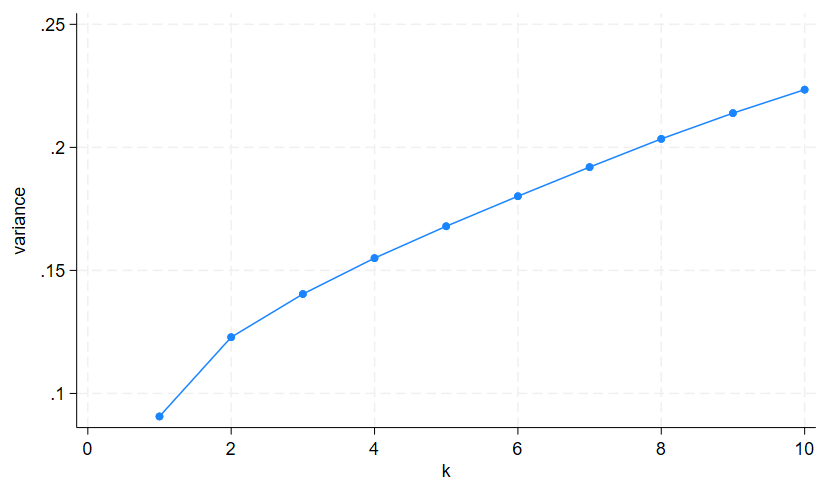
\includegraphics[width=0.5\linewidth]{./Figures/norway_income_change_variance.png}
%
%    Source: SSB (Elin Halvorsen)
%  \end{center}
%  Also see Crawley, Holm, and Tretvoll (2024)
%\end{frame}

\begin{frame}
  \frametitle{Preferences, Beliefs, and Wealth}
  Infinite horizon model: target wealth depends on `Growth Impatience' condition:
\begin{equation}
  \underbrace{
    \left(
      \frac{(\Rfree \; \DiscFac^{e,i})^{1/\gamma}}
      {\PermGroFac^{e} \; \Ex[\permShk^{-1}]}
    \right)
    }_{\text{'Growth Patience Factor'}}
      < 1
    \end{equation}
    
  \pause 
  \emph{Degree} of impatience (1-GPF) determines \emph{size} of target
  \begin{itemize}[<+->]
	\item If everybody has same GPF, then target wealth is identical
	\item Fact: Wealth much more unevenly distributed than permanent income \\[1ex]
		 $\Rightarrow$ need heterogeneity in GPF
	\item (If GPF $\geq 1$, target is $\infty$)
  \end{itemize}

  \hypertarget{ConsistentWithMicroData}{}

  \pause
  We use
  \begin{itemize}[<+->]
  \item \textit{Ex-ante} heterogeneity in discount factors $\DiscFac^{e,i}$
  \item $\PermGroFac^{e}$ or $\Rfree$ would do as well
  \end{itemize}
  
\end{frame}

\begin{frame}
  \frametitle{Consistency With Micro Evidence (1)}
  \begin{columns}
    \begin{column}{0.3\linewidth}
      Liquid Wealth from \href{https://www.federalreserve.gov/econres/scfindex.htm}{Survey of Consumer Finances (SCF)}
	\end{column}	
	\begin{column}{0.7\linewidth}
	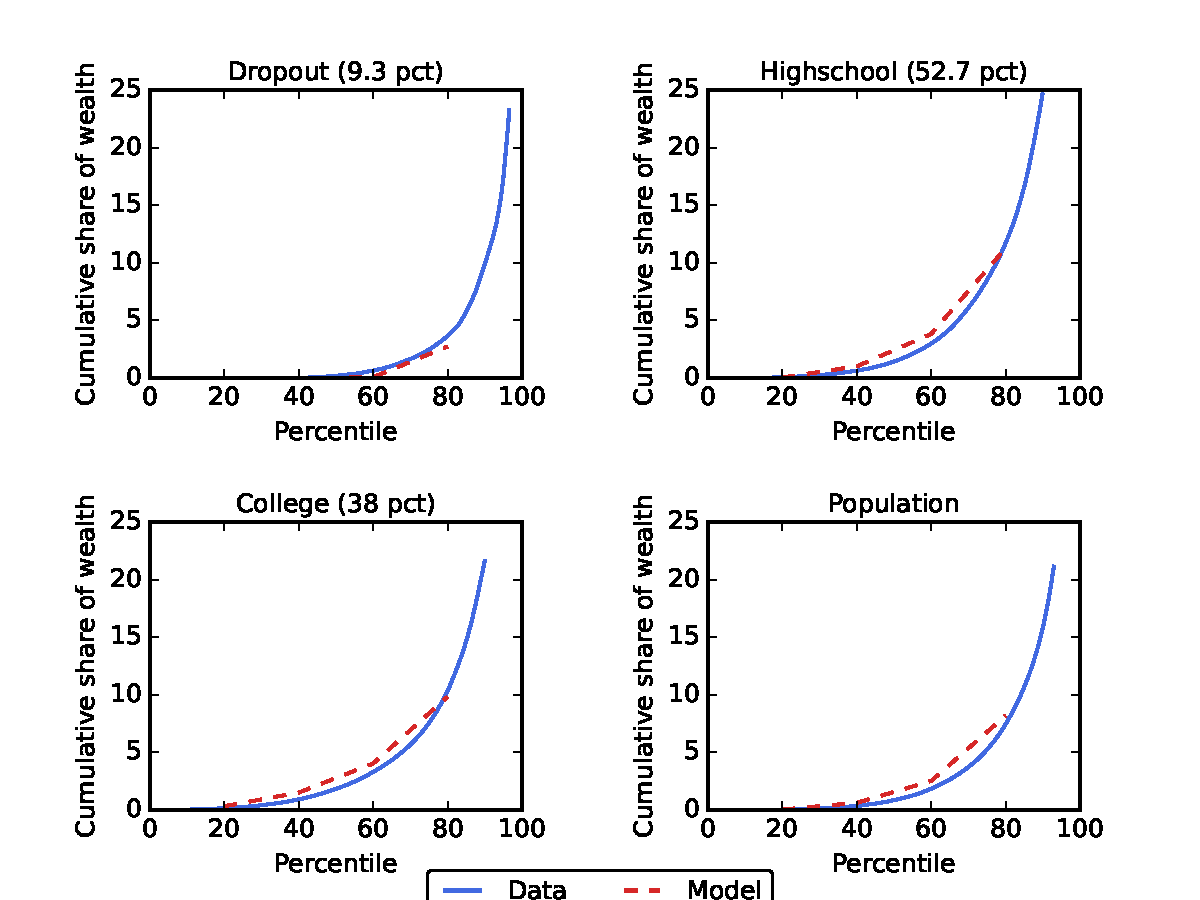
\includegraphics[width=.9\linewidth]{\FigDir/LorenzPoints}
    \end{column}
 \end{columns}
\medskip 
\begin{itemize}
	\item Education groups: $e\in\{$"Dropout", "Highschool" and "College"$\}$
	\item Each group has distribution of discount factors $\beta_{e,i}$
\end{itemize}	
\end{frame}

\begin{frame}
	\frametitle{Consistency With Micro Evidence (2)}
% \begin{columns}
%		\begin{column}{0.4\textwidth}  	
			Intertemporal MPC from Fagereng, Holm, Natvik (2021)
			\begin{center}
			\includegraphics[width=.55\linewidth]{\econtexRoot/Code/HA-Models/Target_AggMPCX_LiquWealth/Figures/AggMPC_LotteryWin}
			\end{center}			
			Modeling device: `Splurge' in consumption
%		\end{column}
%	\end{columns}
\end{frame}


\begin{frame}
\frametitle{Splurge consumption}
\begin{itemize}
	\itemsep = .75\bigskipamount 
	\item Exogenous fraction of income directly consumed
	\item Model consistent with spending patterns over time after a transitory income shock
	\item Evidence: High liquid wealth hh also have high MPCs
	\begin{itemize}
		\itemsep = .25\bigskipamount 
		\item Kueng (2018); Crawley and Kuchler (2023); Graham and McDowall (2024) 
	\end{itemize}
	\item Possible microfoundations: 
	\begin{itemize}
	\itemsep = .25\bigskipamount 
	\item Spending on durables (Browning and Crossley, 2009; Laibson et al., 2022)
	\item A form of present bias (Indarte et al., 2024, Maxted et al., 2024)
	\end{itemize}
	\item Robustness: Model w/o splurge consumption 
\end{itemize}
\end{frame}


    \begin{frame}
      \frametitle{Evaluation of consumption stimulus policies in the US}
      \begin{itemize}[<+->]
        \itemsep = .5\bigskipamount 
      \item Policies we consider: 
        \begin{itemize}[<+->]
          \itemsep = .25\bigskipamount 
        \item Stimulus check for \$1200 (means-tested)
        \item Extension of unemployment benefits from 6 months to 1 year
        \item Payroll tax cut by 2\% for 2 years
        \end{itemize}
        \medskip
        \item Motivation: 
        \begin{itemize}[<+->]
       	  \itemsep = .25\bigskipamount
       	\item Economic Stimulus Act of 2008 (stimulus checks)
       	\item Tax Relief, Unemployment Insurance Reauthorization, and Job Creation Act of 2010 (UI extension and tax cut)
       	\end{itemize}
        % \item Key features of the policies: 
        %   \begin{itemize}[<+->]
        %     \itemsep = .25\bigskipamount 
        %   \item Targeting 
        %   \item Timing of spending (overlap with recession!)
        %   \item Scalability 
        %   \end{itemize}
        \medskip
      \item Evaluation criteria: 
        \begin{itemize}[<+->]
          \itemsep = .25\bigskipamount 
        \item Spending multipliers
        \item Welfare (only recession-related welfare impact)
        \end{itemize}
      \end{itemize}
    \end{frame}


    \begin{frame}
      \frametitle{Preview of results}
      \begin{itemize}[<+->]
        \itemsep = \bigskipamount 
      \item Welfare measure: Extension of UI benefits is the clear winner 
        \begin{itemize}[<+->]
          \itemsep = .25\bigskipamount 
        \item Targeted at individuals with high MPCs and high recession-related welfare losses
        \item But: higher spending may continue after recession is over 
        \end{itemize}
      \item Spending multiplier: Stimulus check has the highest multiplier 
        \begin{itemize}[<+->]
          \itemsep = .25\bigskipamount 
        \item Not well targeted, but increases income immediately 
          % \item Also: easy to scale up
        \end{itemize}
      \item Tax cut
        \begin{itemize}[<+->]
          \itemsep = .25\bigskipamount 
        \item Poorly targeted and much spending likely to occur after end of recession
        \end{itemize}
      \item Robustness in a HANK and SAM model
      	\begin{itemize}[<+->]
      		\itemsep = .25\bigskipamount 
      	\item Very similar pattern for cumulative multipliers 
      	\end{itemize}
      \end{itemize}
    \end{frame}



    \section{Model}

    \begin{frame}
      \frametitle{Household problem}
      \begin{itemize}[<+->]
      \item Idiosyncratic, stochastic income process $\mathbf{y}_{i,t}$
      \item Estimated splurge factor $\varsigma$: $\mathbf{c}_{sp,i,t} = \varsigma \mathbf{y}_{i,t}$
        \pause
      \item Remaining consumption $c_{opt,i,t}$ is chosen to maximize utility
        \begin{equation}\begin{gathered}\begin{aligned}
          \sum_{t=0}^{\infty}\beta_{e,i}^t (1-D)^t \mathbb{E}_0 u(\mathbf{c}_{opt,i,t}).
        \end{aligned}\end{gathered}\end{equation}
        ($D$: end-of-life probability, $u$: CRRA utility function)	
      \item Budget constraint, given existing market resources $\mathbf{m}_{i,t}$ and income state, and a no-borrowing constraint: 
        \begin{equation}\begin{gathered}\begin{aligned}
          \mathbf{m}_{i,t+1} &= R \underbrace{(\mathbf{m}_{i,t} - \mathbf{c}_{sp,i,t} - \mathbf{c}_{opt,i,t})}_{\geq 0 \text{ (no-borrowing constraint)}} + \mathbf{y}_{i,t+1}
        \end{aligned}\end{gathered}\end{equation}
        ($R$: exogenous gross interest rate)
      \end{itemize}
    \end{frame}


    \begin{frame}
      \frametitle{ Income process}

      \begin{itemize}[<+->]

      \item Income subject to transitory, unempl. and permanent shocks
        \begin{equation}\begin{gathered}\begin{aligned}
          \mathbf{y}_{i,t} =   \begin{cases}
            \xi_{i,t}\mathbf{p}_{i,t}, & \text{if employed} \\
            0.7 \mathbf{p}_{i,t}, & \text{if unemployed for $\leq$ 2q} \\
            0.5 \mathbf{p}_{i,t}, & \text{if unemployed $\ge$ 2q} 
          \end{cases}
        \end{aligned}\end{gathered}\end{equation}
        ($\xi_{i,t}$: trans.
shock, $p$: perm.
income)
        
      \item "Permanent income":  $\mathbf{p}_{i,t+1} = \underbrace{\psi_{i,t+1}}_{\text{perm.
shock}} \underbrace{\Gamma_{e(i)}}_{\text{educ.-specific growth}}\mathbf{p}_{i,t}$ 


        \pause
        \bigskip
%      \item Employment status is subject to a Markov process
%        \begin{itemize}[<+->]
%        \item Unemployment rate education-specific (doubles in recession)
%        \item Expected length of unemployment: 1.5q  (4q in recession)
%        \end{itemize}
%        
%      \item Recession is given by an MIT shock; end of recession as a Bernoulli process (avg.
%length of 6q)

	\item Model is a simplified model of households (no heterogeneity in hh size)
	\item Replacement rates reflect some degree of hh incurance (Rothstein and Valetta, 2017)       
        
      \end{itemize}

    \end{frame}

\begin{frame}
	\frametitle{ Employment status and recessions}
	\begin{itemize}
		\itemsep = \bigskipamount 
		\item Emplyoment status is subject to a Markov process
		\begin{itemize}
			\itemsep = .5\bigskipamount
			\item Employed consumer: continue being employed or become unemployed 
			\item Unemployed consumers: receives benefits for two quarters
		\end{itemize}
		
		\item Bureau of Labor Statistics: Report unemployment rates by education group 
		
		\item Recession is given by an MIT shock
		\begin{itemize}
			\itemsep = .5\bigskipamount
			\item Unemployment rate doubles in each education group
			\item Expected length of unemployment increases from 2 to 4q
			\item End of recession occurs as a Bernoulli process calibrated for an avg. rec. length of 6q
		\end{itemize}
	\end{itemize}
\end{frame}


\begin{frame}
\frametitle{Aggregate demand effects \\ 
	\small (as in Krueger, Mitman and Perri, 2016) \normalsize}
\begin{itemize}[<+->]
	\itemsep = .5\bigskipamount 
	\item Baseline: No feedback from aggregate consumption to income
	\item Extension: We allow for aggregate demand effects from consumption on income during the recession
	
	\item The AD effect is given by
	\begin{equation}\begin{gathered}\begin{aligned}
				AD(C_t) =   \begin{cases}
					\Big(\frac{C_t}{\tilde{C}}\Big)^\kappa, & \text{if in a recession} \\
					1, & \text{otherwise} ,
				\end{cases}
	\end{aligned}\end{gathered}\end{equation}
	where $\tilde{C}$ is the level of consumption in the steady state.
	
	
	\item Idiosyncratic income in the extension model is then given by
	\begin{equation}\begin{gathered}\begin{aligned}
				\mathbf{y}_{AD,i,t} = AD(C_t)\mathbf{y}_{i,t}.
	\end{aligned}\end{gathered}\end{equation}
\end{itemize}
\end{frame}


%\begin{frame}
%	\frametitle{Three policies to fight the recession - Details}
%	
%	\begin{itemize}[<+->]
%		\item Stimulus check
%		\begin{itemize}[<+->]
%			\item Everyone receives a check for \$1,200 in q1 of the recession
%			\item Check is means-tested: Full check if perm. income $\leq$ \$100k; Falls linearly for higher incomes and zero for those $\geq$ \$150k
%		\end{itemize}
%		
%		\item Extended unemployment benefits
%		\begin{itemize}[<+->]
%			\item Unemployment benefits are extended from 2 to 4 q
%			\item Extension occurs regardless of whether recession ends
%		\end{itemize}
%		
%		\item Payroll tax cut
%		\begin{itemize}[<+->]
%			\item Employees payroll tax rate is reduced such that income rises by 2\% for 8q	
%		\end{itemize}
%	\end{itemize}
%	
%	Policies are debt-financed and repayed much later
%\end{frame}


\begin{frame}
	\frametitle{Parameters --- by education group \hyperlink{sli:paramsSame}{\beamerbutton{More parameters}} \hyperlink{sli:policies}{\beamerbutton{Policy parameters}}}
	\label{sli:paramsByEd}
	\hypertarget{Parameters}{}
	\begin{tabular}{lccc}
		\toprule 
		\multicolumn{4}{l}{Parameters calibrated for each education group} \\ \midrule
		& Dropout & Highschool & College \\ \midrule
		Percent of population & \phantom{0}9.3 & 52.7 & 38.0 \\ 
		Avg. quarterly PI of ``newborn'' agent (\$1000) & \phantom{0}6.2 & 11.1 & 14.5 \\
		Std. dev. of $\log($PI$)$ of ``newborn'' agent & 0.32 & 0.42 & 0.53 \\
		Avg. quarterly gross growth rate of PI ($\Gamma_e$) & 1.0036 & 1.0045 & 1.0049 \\[1.5ex]
		Unemployment rate in normal times (percent) & \phantom{0}8.5 & \phantom{0}4.4 & \phantom{0}2.7 \\ 
		Probability of entering unemployment ($\pi_{eu}^{e}$, percent) & \phantom{0}6.2 & \phantom{0}3.1 & \phantom{0}1.8 \\
		Probability of leaving unemployment ($\pi_{ue}$) & 0.667 & 0.667 & 0.667 
		\\ \bottomrule 
	\end{tabular}
\begin{itemize}
	\item Mincer (1991) and Elsby and Hobjin (2010): Education groups differ in the incidence of unemployment, not its duration 
\end{itemize}
\end{frame}






    \ifbool{fullcon}{

        \section{Parametrization}

        \begin{frame}
          \frametitle{Parametrization --- Strategy}
          \begin{itemize}[<+->] 
            \itemsep = \bigskipamount 
          \item Step 1: Estimate the splurge factor in a Norwegian version of the economy --- match iMPCs from FHN (2021)
          \item Step 2a: Calibrate a set of parameters that affect all education groups equally 
          \item Step 2b: Calibrate a set of parameters that match features of the different education groups 
          \item Step 3: Estimate a discount factor distribution for each education group to match within-group distribution of liquid wealth
            \begin{itemize}[<+->]
              \itemsep = .25\bigskipamount 
            \item $\beta_e$: center of discount factor distribution
            \item $\nabla_e$: spread of discount factor distribution 
            \item Uniform distribution, approximated with 7 different types
            \end{itemize}
          \end{itemize} 
        \end{frame}

        \begin{frame}
          \frametitle{Step 1: iMPC from FHN (2021)}
          \centering 
          %	\includegraphics[width=3in]{\FigDir/AggMPC_LotteryWin}
          \includegraphics[width=3in]{\econtexRoot/Code/HA-Models/Target_AggMPCX_LiquWealth/Figures/AggMPC_LotteryWin}
          \begin{itemize}[<+->]
            \itemsep = .5\bigskipamount 
          \item Estimated splurge factor: $\varsigma = 0.31$; MPC across wealth distrubtion and K/Y untargeted but close to targets
          \item Zero splurge ($\varsigma = 0$): cannot match iMPC, wealth-dep. MPCs and K/Y-ratio at the same time
          \end{itemize}
        \end{frame}

        \begin{frame}
          \frametitle{Parameters --- same for all types  \hyperlink{sli:policies}{\beamerbutton{Policy parameters}} }
          \hypertarget{Parameters}{}
          \begin{tabular}{lcd{3}} 
            \toprule
            \multicolumn{3}{l}{Parameters that apply to all types} \\ \midrule	
            Parameter & Notation & \text{Value} \\ \midrule 
            Risk aversion & $\gamma$ & 2.0 \\ 
            Splurge & $\varsigma$ & 0.306 \\ 
            Survival probability, quarterly & $1-D$ & 0.994 \\
            Risk free interest rate, quarterly (gross) & $R$ & 1.01 \\ 
            Standard deviation of transitory shock & $\sigma_\xi$ & 0.346 \\
            Standard deviation of permanent shock & $\sigma_\psi$ & 0.0548 \\ 
            Unemployment benefits replacement rate (share of PI) & \textcolor{red}{$\rho_b$} & \textcolor{red}{0}.\textcolor{red}{7} \\ 
            Unemployment income w/o benefits (share of PI) & \textcolor{red}{$\rho_{nb}$} & \textcolor{red}{0}.\textcolor{red}{5} \\ 
            Avg. duration of unemp. benefits in normal times (quarters) & & 2 \\
            Avg. duration of unemp. spell in normal times (quarters) & & 1.5 \\
            Probability of leaving unemployment & $\pi_{ue}$ & 0.667 \\ 
            Consumption elasticity of aggregate demand effect & $\kappa$ & 0.3 
            \\ \bottomrule 
          \end{tabular}
        \end{frame}


        \begin{frame}
          \frametitle{Step 2b: Parameters --- by education group}
          \label{sli:paramsByEd}
          \begin{tabular}{lccc}
            \toprule 
            \multicolumn{4}{l}{Parameters calibrated for each education group} \\ \midrule
            & Dropout & Highschool & College \\ \midrule
            Percent of population & \phantom{0}9.3 & 52.7 & 38.0 \\ 
            Avg. quarterly PI of ``newborn'' agent (\$1000) & \phantom{0}6.2 & 11.1 & 14.5 \\
            Std. dev. of $\log($PI$)$ of ``newborn'' agent & 0.32 & 0.42 & 0.53 \\
            Avg. quarterly gross growth rate of PI ($\Gamma_e$) & 1.0036 & 1.0045 & 1.0049 \\
            Unemployment rate in normal times (percent) & \phantom{0}8.5 & \phantom{0}4.4 & \phantom{0}2.7 \\ 
            Probability of entering unemployment ($\pi_{eu}^{e}$, percent) & \phantom{0}6.2 & \phantom{0}3.1 & \phantom{0}1.8 
            \\ \bottomrule 
          \end{tabular}
        \end{frame}


        \begin{frame}
          \frametitle{Step 3: Estimation of discount factors}
          \begin{tabular}{lccc}
            & Dropout & Highschool & College \\ \midrule
            $(\beta_e, \nabla_e)$ & (0.735, 0.298) & (0.924, 0.137) & (0.984,0.010) \\
            (Min, max) in approximation & (0.480, 0.991) & (0.806, $0.989^*$) & (0.976, 0.992) \\
            \midrule 
          \end{tabular} 
          \begin{tabular}{lccc}
            \multicolumn{4}{l}{ } \\ \midrule
            \textbf{Estimation targets} & Dropout & Highschool & College \\ \midrule
            Median LW/ quarterly PI (data, percent) & 4.64 & 30.2 & 112.8 \\ 
            Median LW/ quarterly PI (model, percent) & 4.64 & 30.2 & 112.8 %\\
            % $[20,40,60,80]$ pctiles of Lorenz curve (data) & $[0, 0.01, 0.6, 3.6]$ & $[0.06, 0.6, 3.0, 11.6]$ & $[0.2, 0.9, 3.3, 10.3]$ \\
            % $[20,40,60,80]$ pctiles of Lorenz curve (model) & $[0.0, 0.0, 0.5, 3.6]$ & $[0.04, 0.9, 3.7, 11.3]$ & $[0.3, 1.5, 4.0, \phantom{0}9.9]$
            \\ \midrule 
          \end{tabular} 
          \begin{tabular}{lcccc}
            \multicolumn{5}{l}{ } \\ \midrule
            \textbf{Non-targeted moments} & Dropout & Highschool & College & Population \\ \midrule
            Percent of total wealth (data) & 0.8 & 17.9 & 81.2 & 100 \\
            Percent of total wealth (model) & 1.1 & 21.9 & 77.0 & 100 \\
            Avg. annual MPC (model, incl. splurge) & 0.87 & 0.71 & 0.48 & 0.64
            \\ \bottomrule 
          \end{tabular}
        \end{frame}




        \begin{frame}
          \frametitle{Step 3: Visualization of match with SCF}
          \centering
          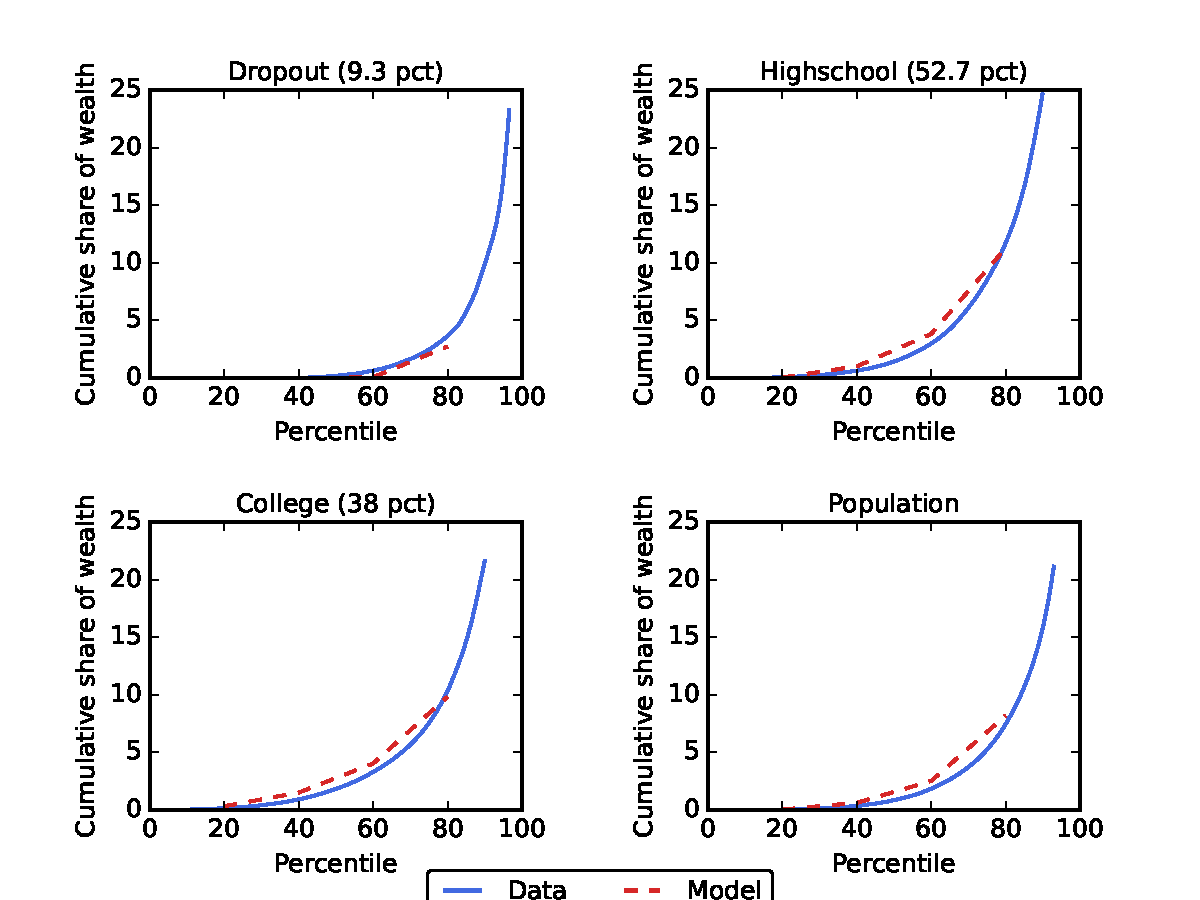
\includegraphics[width=4in]{\FigDir/LorenzPoints}
        \end{frame}


      }{}

      \section{Results}


      \ifbool{bundesb}{

          \begin{frame}
            \frametitle{Impulse responses}


            \begin{columns}	
              
              
              \begin{column}{0.5\textwidth} 
                \small 	
                \begin{itemize}[<+->]
                \item Simulate policies in recessions lasting 1 to 20 q
                \item Construct probability-weighted sum across rec. lengths
                \end{itemize}
              \end{column}	
              
              
              \begin{column}{0.4\textwidth}  
                \footnotesize Stimulus check:
                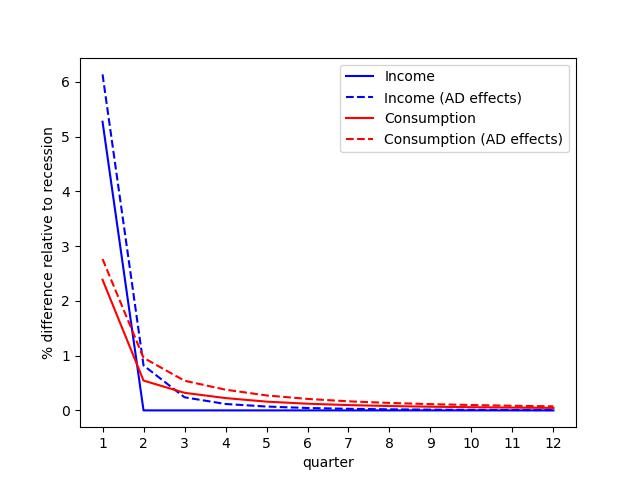
\includegraphics[width=\linewidth]{\econtexRoot/Code/HA-Models/FromPandemicCode/Figures/recession_Check_relrecession}
                
              \end{column}  	

            \end{columns}

            \pause
            
            \begin{columns}	
              
              \begin{column}{0.33\textwidth}  	
                \footnotesize Extension of UI benefits:
                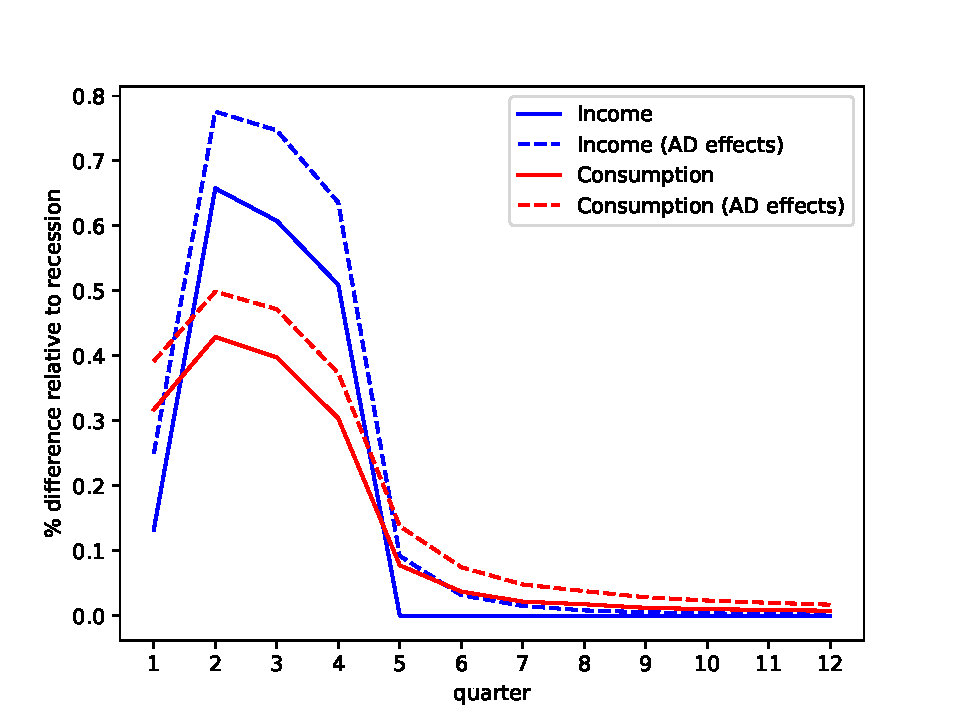
\includegraphics[width=1.2\linewidth]{Code/HA-Models/FromPandemicCode/Figures/recession_UI_relrecession} 
              \end{column}
              
              \begin{column}{0.33\textwidth}  
                \footnotesize Payroll tax cut:	
                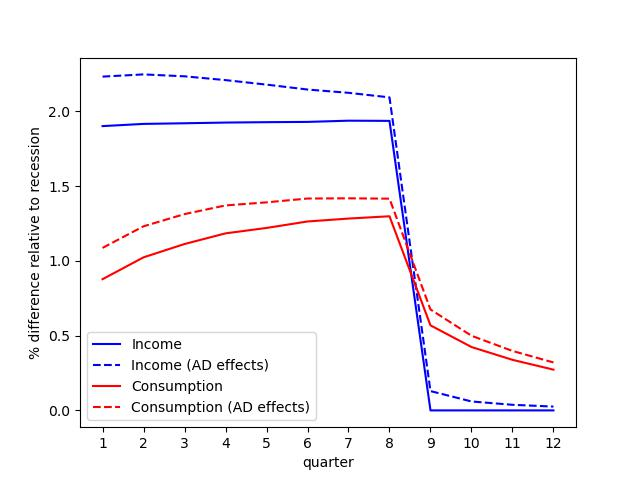
\includegraphics[width=1.2\linewidth]{Code/HA-Models/FromPandemicCode/Figures/recession_taxcut_relrecession}
              \end{column}
            \end{columns}

          \end{frame}
        }{}



        \ifbool{fullcon}{
            
            
            
            


            \begin{frame}
              
              \frametitle{IRFs for stimulus check}
              
              \begin{columns}	
                
                \begin{column}{0.33\textwidth} 	
                  \begin{itemize}[<+->]
                  \item Simulate check policy in recessions lasting  from 1 to 20 q
                  \item Construct probability-weighted sum across rec. lengths
                  \end{itemize}
                \end{column}	
                
                
                \begin{column}{0.66\textwidth}  
                  \centering
                  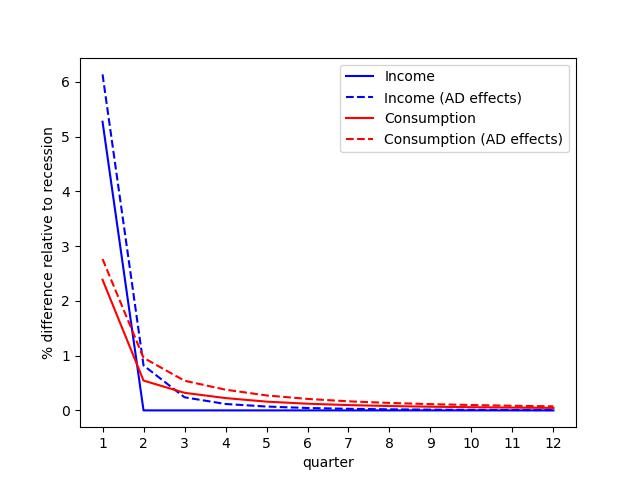
\includegraphics[width=\linewidth]{\econtexRoot/Code/HA-Models/FromPandemicCode/Figures/recession_Check_relrecession}
                \end{column}  
                
              \end{columns}

            \end{frame}

            \begin{frame}
              \frametitle{IRfs for extension of unemployment benefits / payroll tax cut}

              \begin{columns}	
                
                \begin{column}{0.50\textwidth}  	
                  Extension of UI benefits:
                  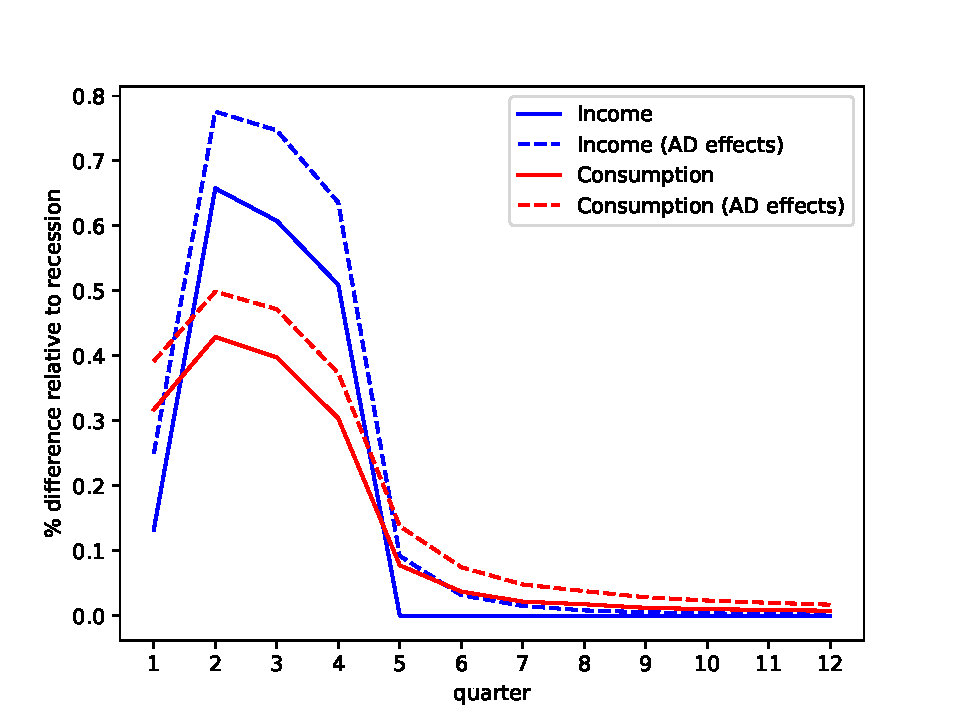
\includegraphics[width=1.2\linewidth]{Code/HA-Models/FromPandemicCode/Figures/recession_UI_relrecession} 
                \end{column}
                
                \begin{column}{0.50\textwidth}  
                  Payroll tax cut:	
                  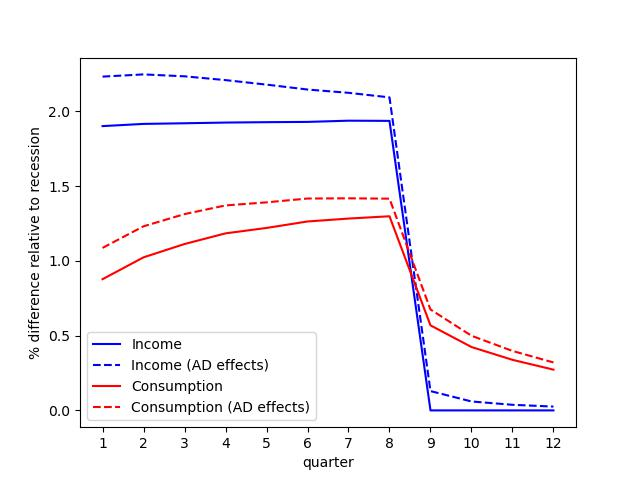
\includegraphics[width=1.2\linewidth]{Code/HA-Models/FromPandemicCode/Figures/recession_taxcut_relrecession}
                \end{column}
              \end{columns}
              
            \end{frame}
            
          }{}


\begin{frame}
\frametitle{Untargeted moments (1)}
\begin{tabular}{lcccc}
	\multicolumn{5}{l}{Non-targeted moments by wealth quartile} \\ \midrule
	& WQ 4 & WQ 3 & WQ 2 & WQ 1 \\ \midrule
	Percent of liquid wealth (data) & 0.14 & 1.60 & 8.51 & 89.76 \\
	Percent of liquid wealth (model, baseline) & 0.09 & 0.96 & 4.55 & 94.40 \\
	\textcolor{gray}{Percent of liquid wealth (model, Splurge=0)} & \textcolor{gray}{0.10} & \textcolor{gray}{1.07} & \textcolor{gray}{4.24} & \textcolor{gray}{94.60} \\
	\makecell[l]{Avg. lottery-win-year MPC \\ (model, incl. splurge)} & 0.78 & 0.63 & 0.44 & 0.31 \\
	\makecell[l]{\textcolor{gray}{Avg. lottery-win-year MPC} \\ \textcolor{gray}{(model, splurge=0)}} & \textcolor{gray}{0.69} & \textcolor{gray}{0.53} & \textcolor{gray}{0.36} & \textcolor{gray}{0.14}
	\\ \bottomrule 
\end{tabular}
\end{frame}

\begin{frame}
\frametitle{Untargeted moments (2)}
\begin{columns}
	\begin{column}{0.50\textwidth}
		\begin{figure}
			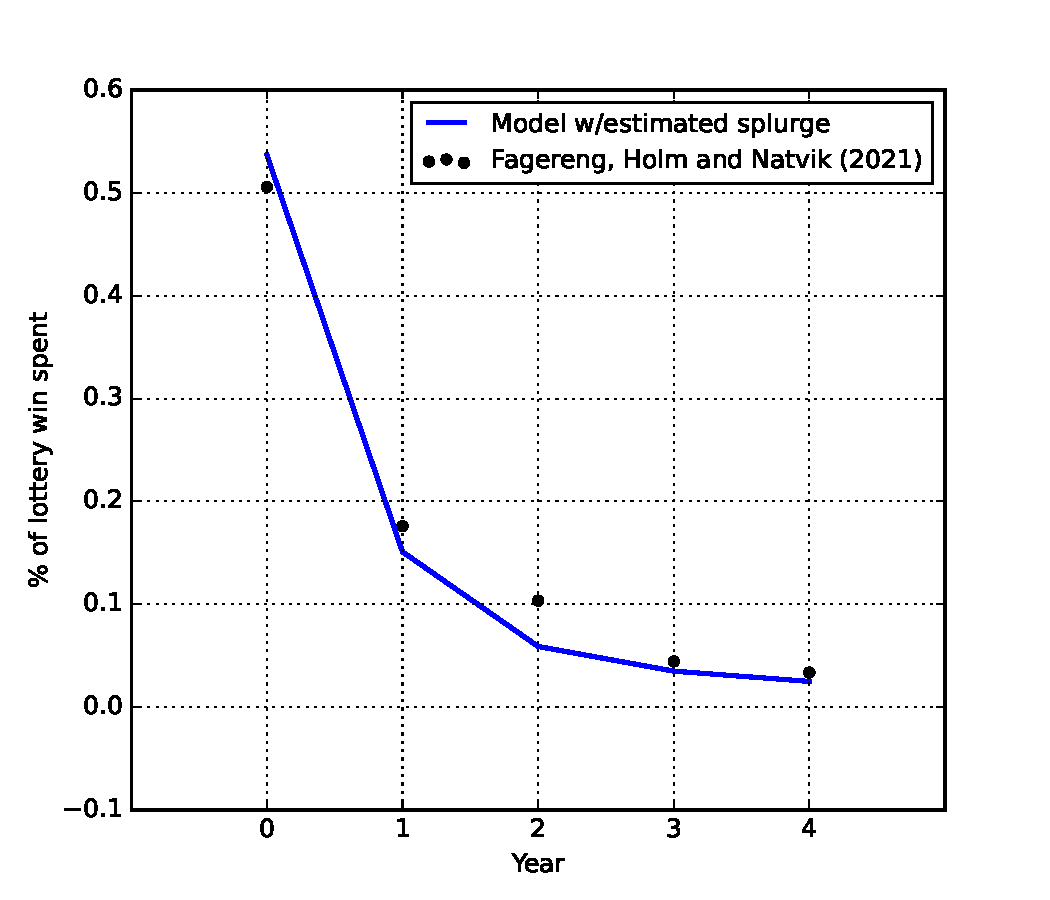
\includegraphics[width=.9\linewidth]{\econtexRoot/Figures/IMPCs_wSplEstimated}
			\caption{Share of lottery win spent}
		\end{figure}
	\end{column}
	\begin{column}{0.50\textwidth}
		\begin{figure}
			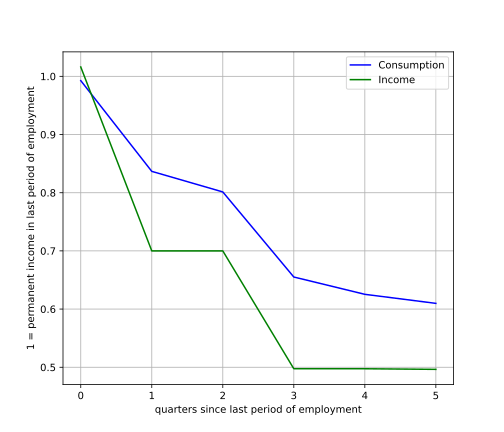
\includegraphics[width=.9\linewidth]{\econtexRoot/Code/HA-Models/FromPandemicCode/Figures/UnempSpell_Dynamics}
			\caption{Spending upon expiry of UI benefits}
		\end{figure}
	\end{column}
\end{columns}
\begin{itemize}
	\item Ganong and Noel (2019): UI expiry $\Rightarrow$ drop of 12 percent (month)
	\item Our model $\Rightarrow$ drop of 18 percent (quarter) 
\end{itemize}
\end{frame}


\begin{frame}
\frametitle{Multipliers}

    \begin{columns}

      \begin{column}{0.50\textwidth}
        \begin{equation*}
          M^P_t = \frac{\text{NPV of induced consumption up to $t$}}{\text{NPV of the cost of the policy}}
        \end{equation*}
      \end{column}

      \begin{column}{0.50\textwidth}

        \begin{figure}[t]
          \centering
          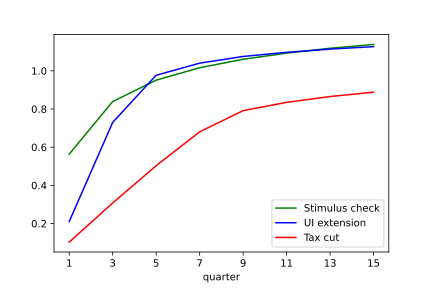
\includegraphics[width=\linewidth]{Code/HA-Models/FromPandemicCode/Figures/Cummulative_multipliers}
        \end{figure}

      \end{column}
    \end{columns}

    \begin{table}[t]
      \begin{tabular}{@{}lccc@{}} 
        \toprule 
        & Stimulus check    & UI extension    & Tax cut     \\  \midrule 
        10y-horizon Multiplier (no AD effect) &0.85  & 0.89  & 0.83     \\ 
        10y-horizon Multiplier (AD effect) &1.20  & 1.18  & 0.95     \\ 
        % 10y-horizon (1st round AD effect only) &1.162  & 1.140  & 0.967     \\ 
Share of policy expenditure during recession &100.0\%  & 80.6\%  & 57.6 \%    \\ 
\end{tabular}  
\end{table}
\end{frame}

\begin{frame}
\frametitle{Robustness: Multipliers in a HANK and SAM model --- Setup}
\begin{itemize}
\itemsep = .5\bigskipamount 
\item Evaluate the policies in a relatively standard HANK and SAM model (Du, 2024)
\item New Keynesian: Monopolistic competition + sticky prices
\item Search and matching: Random search, labor market tightness affects job finding and vacancy filling probabilities 
\item Government policy: Monetary and fiscal rules 
\item Fiscal multipliers through an intertemporal Keynesian cross mechanism \\[1ex]
However: No state dependence 
\item Solution method $\Rightarrow$ cannot evaluate effects starting in a deep recessionary state \\[1ex]
This also implies that we cannot use our welfare measure 
\end{itemize}
\end{frame}

\begin{frame}
\frametitle{Robustness: Multipliers in a HANK and SAM model --- Results}
\begin{figure}
\begin{center}
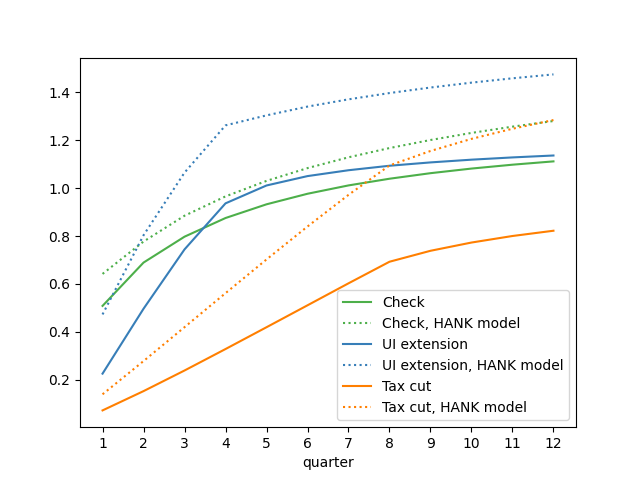
\includegraphics[scale=0.6]{Code/HA-Models/FromPandemicCode/Figures/Cummulative_multipliers_withHank}	
\end{center}
\vspace{0.2cm}
\captionof{figure}{HA w/AD effects + HANK and SAM}
%\hfill
%\begin{minipage}[c]{0.48\linewidth}
%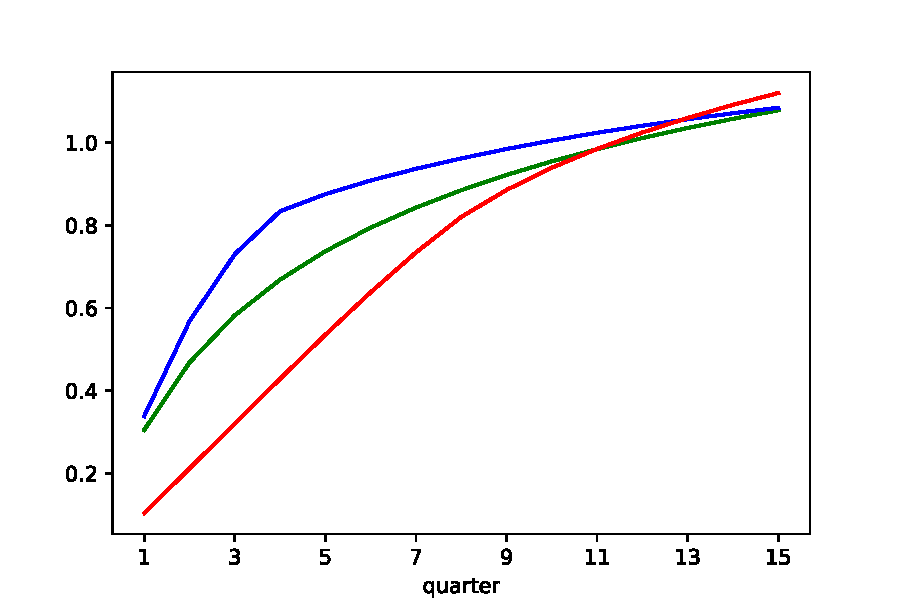
\includegraphics[scale= 0.5]{Code/HA-Models/FromPandemicCode/Figures/Cumulative_multipliers_HANK}
%\vspace{0.2cm}
%\captionof{figure}{HANK XXupdate}
%\end{minipage}
\end{figure}
\end{frame}

\begin{frame}
\frametitle{Welfare measure}
\begin{itemize}[<+->]
\item Aim: Welfare measure does not reflect benefits of redistribution in ``normal'' times
\item Want: Utility-based measure of benefits of implementing a policy in a recession
\item Welfare weights: $u'(\mathbf{c}_{it,\textit{normal}})$
\item Measure for a given $policy$ with $Rec,AD\in\{0,1\}$
\begin{equation}\begin{gathered}\begin{aligned}
& \mathcal{W}(\text{policy},Rec,AD) =\frac{1}{\mathcal{N}} \sum_{i=1}^{N} \sum_{t=0}^{\infty} \frac{1}{R^t} \frac{u(\mathbf{c}_{it,\textit{policy},Rec,AD}) - u(\mathbf{c}_{it,\textit{none},Rec,AD})}{ u'(\mathbf{c}_{it,\textit{normal}})} \\ \\ 
& \mathcal{N} = NPV(\text{policy},Rec,AD)
\end{aligned}\end{gathered}\end{equation}
\item Normal times: $\mathcal{W}(\text{policy},0,0) = 1$ (for $\Delta \mathbf{c}_{it}\approx 0$)
\end{itemize}
\end{frame}

\begin{frame}
	\frametitle{Welfare results}
	\centering 
	\begin{tabular}{@{}lccc@{}} 
		\toprule 
		& Stimulus check      & UI extension    & Tax cut    \\  \midrule 
		$\mathcal{W}(\text{policy}, Rec=0, AD=0)$ & 0.96  & 0.85  & 0.99     \\ 
		$\mathcal{W}(\text{policy}, Rec=1, AD=0)$ & 0.99  & 1.82  & 0.98     \\ 
		$\mathcal{W}(\text{policy}, Rec=1, AD=1)$ & 1.34  & 2.11  & 1.10     \\ \bottomrule
	\end{tabular} 
		\medskip
\begin{itemize}[<+->]
  \itemsep = .75\bigskipamount 
\item Normal times: Welfare of UI extension $< 1$ due to concavity of $u(\cdot)$ \\[1ex] 
Relatively large change in $\mathbf{c}_{it}$ for small number of households 
\item $AD=0$: Benefit of UI extension since recession increases unemployment $\Rightarrow$ increased marginal utility for affected households 
\item $AD=1$: Stimulating spending during recession increases measure for all policies 
\end{itemize}
\end{frame}

\begin{frame}
	\frametitle{Conclusion: Comparing the policies}
	\begin{itemize}[<+->]
		\itemsep = .5\bigskipamount 
		\item Comparison of three consumption stimulus policies in a HA model consistent with data on the distribution of liquid wealth and intertemporal MPCs 
		\item Welfare measure: UI extension is the clear bang-for-the-buck winner 
		\item The stimulus check is less well targeted, but\ldots 
		\begin{itemize}[<+->]
			\itemsep = .25\bigskipamount 
			\item is transferred immediately ensuring that money arrives when it is most valuable 
			\item is more easily scaled up to provide more stimulus 
		\end{itemize}
		\item The tax cut is both poorly targeted and may yield substantial spending after the recession is over 
		\item Framework can be used to evaluate other candidate policies 
		
	\end{itemize}
	
\end{frame}



\begin{frame}
	\frametitle{Thank you for your attention!}
	\begin{itemize}[<+->] 
		\item Access the paper, presentation slides and code at: \href{https://github.com/llorracc/HAFiscal}{https://github.com/llorracc/HAFiscal}
	\end{itemize}	

		\begin{figure}
			\centering
			
\includegraphics[width=0.3\linewidth]{Presentations/qr-code}
		\end{figure}
	
\end{frame}






\section{Appendix}

\begin{frame}
\frametitle{Parameters --- same for all types}
\label{sli:paramsSame}
%\begin{tabular}{lcd{3}} 
\begin{tabular}{lcc}
	\toprule
%	\multicolumn{3}{l}{Parameters that apply to all types} \\ \midrule	
	Parameter & Notation & \text{Value} \\ \midrule 
	Risk aversion & $\gamma$ & 2.0 \\ 
	Splurge & $\varsigma$ & 0.306 \\ 
	Survival probability, quarterly & $1-D$ & 0.994 \\
	Risk free interest rate, quarterly (gross) & $R$ & 1.01 \\ 
	Standard deviation of transitory shock & $\sigma_\xi$ & 0.346 \\
	Standard deviation of permanent shock & $\sigma_\psi$ & 0.0548 \\ 
	Unemployment benefits replacement rate (share of PI) & \textcolor{red}{$\rho_b$} & \textcolor{red}{0}.\textcolor{red}{7} \\ 
	Unemployment income w/o benefits (share of PI) & \textcolor{red}{$\rho_{nb}$} & \textcolor{red}{0}.\textcolor{red}{5} \\ 
	Avg. duration of unemp. benefits in normal times (quarters) & & 2 \\
	Avg. duration of unemp. spell in normal times (quarters) & & 1.5 \\
%	Probability of leaving unemployment & $\pi_{ue}$ & 0.667 \\ 
	Consumption elasticity of aggregate demand effect & $\kappa$ & 0.3 
	\\ \bottomrule 
\end{tabular}

\vspace{.5cm}
\hyperlink{Parameters}{\beamerbutton{Go back}} 
\end{frame}


\begin{frame}
	\frametitle{Parameters describing the policies}
	\label{sli:policies}
	\begin{center}
	\begin{tabular}{lc}
		\toprule 
		\multicolumn{2}{l}{Parameters describing policy experiments} \\ \midrule 
		Parameter & Value \\ \midrule 
		Change in unemployment rates in a recession & $\times 2$ \\ 
		Expected unemployment spell in a recession & 4 quarters \\ 
		Average length of recession & 6 quarters \\ 
		Size of stimulus check & \$1,200 \\ 
		PI threshold for reducing check size & \$100,000 \\ 
		PI threshold for not receiving check & \$150,000 \\ 
		Extended unemployment benefits & 4 quarters \\
		Length of payroll tax cut & 8 quarters \\ 
		Income increase from payroll tax cut & 2 percent \\ 
		Belief (probability) that tax cut is extended & 50 percent 		
		\\ \bottomrule
	\end{tabular}
	\end{center}
	\vspace{.5cm}
	\hyperlink{Parameters}{\beamerbutton{Go back}} 
\end{frame}


\begin{frame}
\frametitle{Robustness: Model w/o splurge consumption}
\begin{columns}
\begin{column}{0.5\textwidth}
	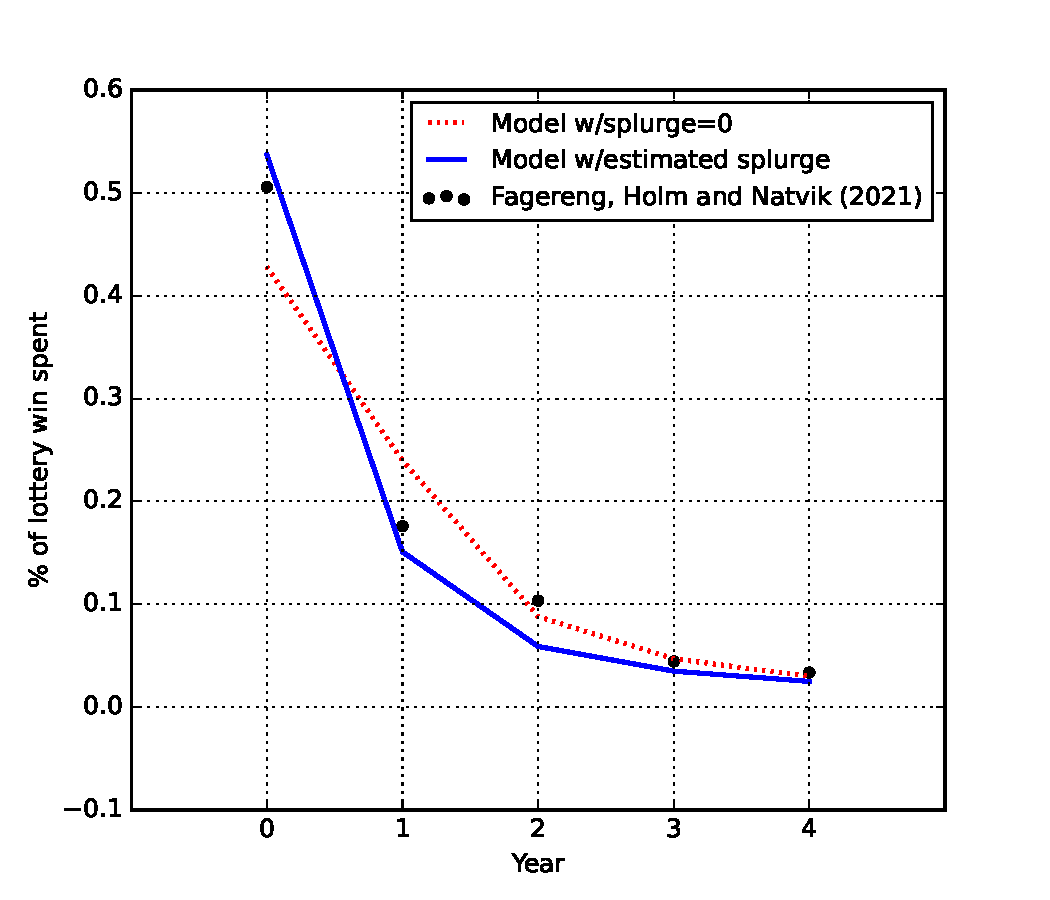
\includegraphics[width=\linewidth]{\econtexRoot/Figures/IMPCs_both}
\end{column}
\begin{column}{0.5\textwidth}
	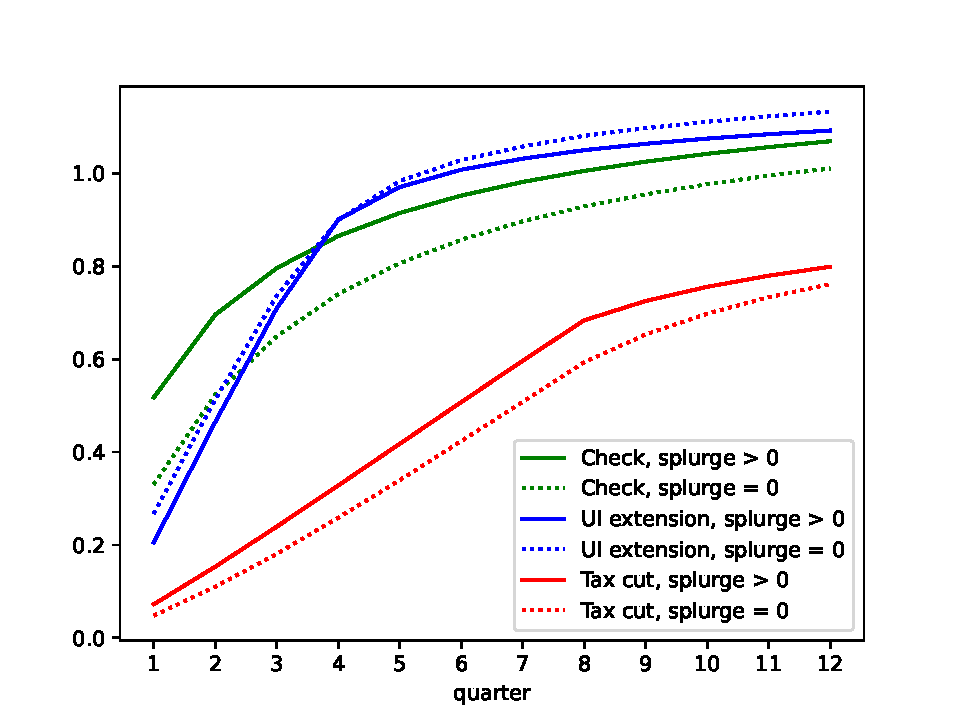
\includegraphics[width=\linewidth]{Code/HA-Models/FromPandemicCode/Figures/Splurge0/Cummulative_multipliers_SplurgeComp}
\end{column}
\end{columns}
\begin{center}
\begin{tabular}{@{}lccc@{}} 
	\toprule 
	& Stimulus check      & UI extension    & Tax cut    \\  \midrule 
%	$\mathcal{W}(\text{policy}, Rec=0, AD=0)$ & 0.97(0.96)  & 0.84(0.85)  & 0.99(0.99)     \\ 
%	$\mathcal{W}(\text{policy}, Rec=1, AD=0)$ & 1.00(0.99)  & 1.80(1.82)  & 0.97(0.98)     \\ 
	$\mathcal{W}(\text{policy}, Rec=1, AD=1)$ & 1.27(1.34)  & 2.12(2.11)  & 1.09(1.10)     \\ \bottomrule
\end{tabular} 
\end{center}
\end{frame}



\end{document}
